\section{Model Parameters and Implementation Notes}
\label{app:params}
Table \ref{tab:params} lists the default parameters used throughout. The array
draws $R_\mathrm{on}$ and $R_\mathrm{off}$ from log-normal distributions (so
resistances stay positive) and the thresholds from clipped Gaussians. The
small-signal read conductance at $V_\mathrm{read}$ is
$G_\mathrm{read}=I(V_\mathrm{read},w)/V_\mathrm{read}$, which is monotonic in $w$
and used for all weight reads.

\begin{table}[h]
\caption{Default device, array, and training parameters.}
\label{tab:params}
\centering
\small
\begin{tabular}{lll}
\toprule
Symbol & Meaning & Value \\
\midrule
$R_\mathrm{on}$ & LRS resistance (nominal) & $2\,\mathrm{k}\Omega$, $\sigma{=}15\%$ \\
$R_\mathrm{off}$ & HRS resistance (nominal) & $200\,\mathrm{k}\Omega$, $\sigma{=}30\%$ \\
$V_\mathrm{set}$ & SET threshold & $0.80$ V, $\sigma{=}0.08$ \\
$V_\mathrm{reset}$ & RESET threshold & $0.70$ V, $\sigma{=}0.08$ \\
$k_\mathrm{s},k_\mathrm{r}$ & switching rates & $80$ \\
$V_0$ & HRS nonlinearity scale & $0.45$ V \\
$p$ & window exponent & $4$ \\
$V_\mathrm{read}$ & read voltage & $0.2$ V \\
-- & cycle-to-cycle noise & $5\%$ \\
$[g_\mathrm{lo},g_\mathrm{hi}]$ & weight window & $[20,300]\,\mu$S \\
$E_a,\tau_0$ & retention (Arrhenius) & $1.0$ eV, $4.8{\times}10^{-9}$ s \\
$w_\mathrm{eq}$ & retention equilibrium & $0.02$ \\
$H$ & hidden units (spiral MLP) & $64$ \\
$w_\mathrm{max}$ & weight window (training) & $10$ \\
-- & batch size; float LR & $32$; $0.3$ \\
-- & pulse LR; max pulse width & $1.5{\times}10^{-3}$; $3{\times}10^{-3}$ \\
-- & IR-train epochs; LR decay & $350$; $0.992$ \\
$r_w$ & wire resistance (IR-train) & $1\,\Omega$/cell \\
\bottomrule
\end{tabular}
\end{table}

\textbf{IR-drop solver.} For an $N\times M$ array there are $2NM$ node voltages
(a row-wire and a column-wire node per cross-point). Assembly is fully
vectorized: device edges, row-wire edges, and column-wire edges are built as
index arrays, the diagonal is accumulated with \texttt{bincount}, and a single
sparse matrix is factored with \texttt{scipy.sparse.linalg.splu}. The same
factorization is reused for every input vector in a batch, which is what makes
hardware-in-the-loop training affordable.

\textbf{Differential decode.} With input voltages $V_\mathrm{in}=x\,V_\mathrm{read}$
and a differential pair encoding $W$, the recovered pre-activation is
$(I^{+}-I^{-})/(\text{decode scale}\cdot V_\mathrm{read})$, which equals $xW$ in
the ideal case; this identity was used to verify the inference pipeline (ideal
write reproduces the software accuracy in Table \ref{tab:inference}).

\section{Session Provenance Log}
\label{app:session}
Following the project's research protocol, we log what was human direction and
what was AI-assisted execution. The research was conducted as an interactive
session in which the human set the direction at each step and verified outcomes,
and the AI assistant (Claude Code) wrote and debugged the simulation code,
produced the figures, and drafted this manuscript. The work was not a
pre-registered plan; it grew turn by turn, which is why the appendix records the
actual order.

\subsection{Human Direction (verbatim prompts, in order)}
\begin{enumerate}
\item ``explain how neuromorphic memristor works''
\item ``lets say we're using AlOx -- i would like to visualize current-voltage
graph and see a simulation of a single device''
\item ``this is too much, i dont want animations, i want to scientifically
understand how the I-V hysteresis happens and how it helps to retain memory
state''
\item ``can you convert this to a script that simulates device level behaviour
and then create 64x64 crossbar array to see aggregate behaviour''
\item ``add wire-resistance IR-drop via a proper nodal solve (this is where 64x64
vs 128x128 starts to matter), model retention/drift as slow thermal relaxation of
w, run a small YOLO inference layer on the array to quantify accuracy loss from
variability''
\item ``if YOLO is too large, can you pick another demonstrable learning task
that can be shown to converge in this env itself, MNIST is too vanilla, also if
required increase the crossbar dims''
\item ``add retention drift between training and inference to see how fast a
trained network degrades, and train with IR-drop in the forward pass to see
whether the loop can learn around the wire resistance too''
\item ``can you somehow visualize the crossbar array and the weights encoded and
inference happening, like a test time inference''
\item ``run the same animation through the IR-drop forward, or animate the
retention drift''
\item ``generate another viz where the two tiles are receiving signals (how the
inputs are encoded to analog signals), and how the output is generated, visualize
the waveforms over time''
\item ``this viz isnt clear, can we make the efficiency takeaway much more
apparent and clear''
\item ``but i dont see the analog inputs coming into the crossbar array in
parallel''
\item ``treat this entire session as research, capture all the results and
generate a detailed paper, use IEEE format''
\end{enumerate}

\subsection{Mapping of Prompts to Outputs}
Table \ref{tab:provenance} maps each direction to the artifact the assistant
produced and the section of this paper that reports it.

\begin{table}[h]
\caption{Provenance: human direction to AI-produced artifact.}
\label{tab:provenance}
\centering
\small
\begin{tabular}{p{0.6cm}p{4.2cm}p{2.0cm}}
\toprule
Prompt & AI-produced artifact & Reported in \\
\midrule
1 & Conceptual explanation (no code) & -- \\
2 & Interactive device simulator (later set aside per prompt 3) & -- \\
3 & Written derivation of hysteresis and retention & Sec.~\ref{sec:device} \\
4 & \texttt{alox\_crossbar.py}: device model, 64x64 array & Fig.~\ref{fig:device}--\ref{fig:compute} \\
5 & \texttt{crossbar\_advanced.py}: MNA IR-drop, retention, conv + classifier & Fig.~\ref{fig:inference}--\ref{fig:retention}, Tab.~\ref{tab:irdrop} \\
6 & \texttt{crossbar\_learn.py}: in-situ two-spiral learning & Fig.~\ref{fig:insitu} \\
7 & Post-training drift; IR-drop in training loop & Fig.~\ref{fig:drift} \\
8--12 & Visualizations of encoding, MVM parallelism, signal flow & App.~\ref{app:extra} \\
13 & This manuscript & -- \\
\bottomrule
\end{tabular}
\end{table}

\subsection{Surprises and Debugging Insights}
Several non-obvious issues were found and fixed during execution; they are logged
here because they shaped the results.
\begin{itemize}
\item \textbf{Frequency collapse direction.} An early run showed the hysteresis
loop growing rather than shrinking with frequency, because the chosen rates let
the device fully switch at every tested frequency. Spacing the frequencies by
decades exposed the correct monotonic collapse (Fig.~\ref{fig:device}c).
\item \textbf{Inference decode bug.} The classifier first scored at chance
despite an ideal write; the cause was an input-voltage scale factor left out of
the differential decode while the bias was not scaled. Cosine similarity hid the
bug in the convolution check because it is scale invariant.
\item \textbf{Weight-range clipping.} In-situ learning stalled near 80 percent
until the conductance window was widened to encode weights up to about $\pm 8$;
the spiral network needs larger weights than a $\pm 3$ window allows.
\item \textbf{Noise as dither.} Noiseless identical devices stalled under
deterministic nonlinear updates, while cycle-to-cycle noise enabled convergence.
\item \textbf{Surrogate-gradient noise.} Hardware-in-the-loop IR-drop training
oscillated because the backward pass uses an ideal-weight surrogate; a pulse-size
decay schedule settled it (Fig.~\ref{fig:drift}c).
\end{itemize}

\subsection{Division of Labour}
Human contribution: the overall direction (start from device physics, scale to an
array, then add each non-ideality), the specific methodological asks (a proper
nodal solve, drift between training and inference, IR drop inside the training
loop, a non-trivial learning task), the decision to set aside an interactive
demo in favour of a reproducible script, and verification of each result. AI
contribution: implementation of the device and array models, the vectorized MNA
solver, the program-verify and in-situ training loops, all figures, the debugging
listed above, and the drafting of this paper. All numerical results were produced
by the released code and inspected by the human before inclusion.

\section{Additional Visualizations}
\label{app:extra}
Figure \ref{fig:compute} (referenced from Section \ref{sec:res-inf}) shows the
program-and-read of an image into the array and the analog MVM scatter.
Figures \ref{fig:parallel} and \ref{fig:circuit} are stills from animations built
to communicate the in-memory parallelism: the first contrasts the $N\times M$
sequential multiply-accumulate of a von Neumann engine with the single parallel
read of the crossbar; the second shows the analog inputs entering all wordlines
simultaneously and current summing down all bitlines at once.

\begin{figure}[t]
\centering
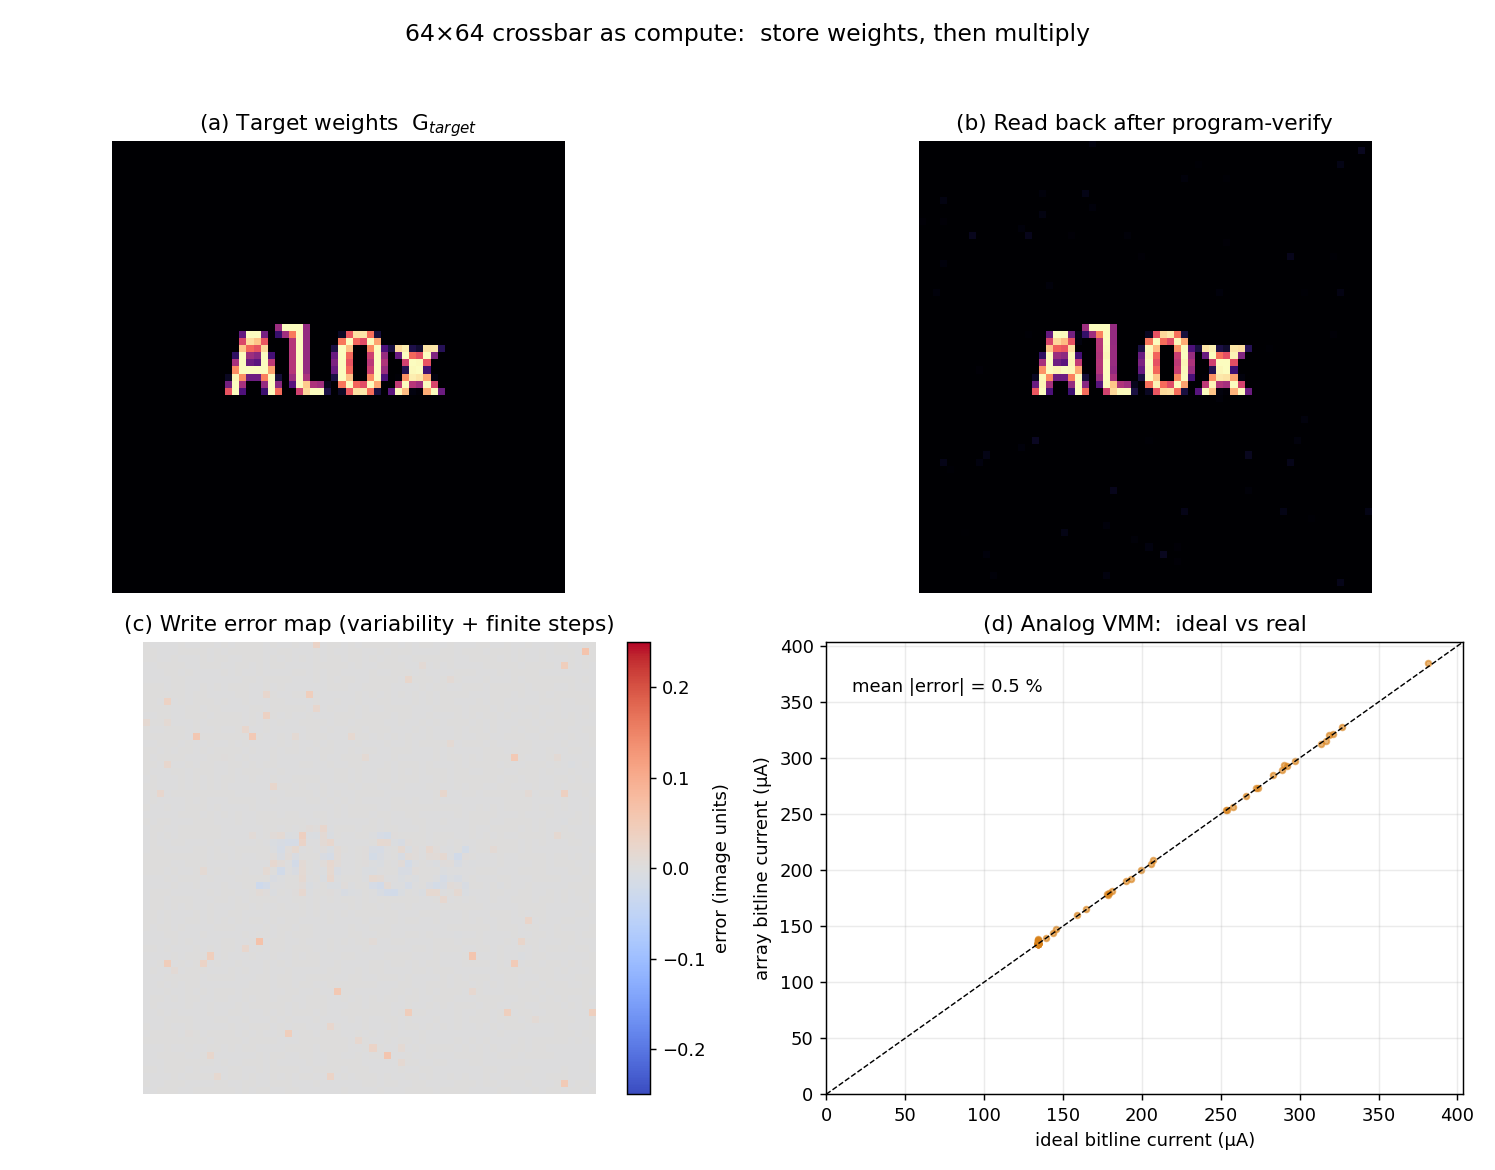
\includegraphics[width=\columnwidth]{figures/fig3_crossbar_compute.png}
\caption{Crossbar as compute. (a) Target weights (an image) and (b) the array
read-back after program-verify. (c) Write-error map. (d) Analog MVM versus ideal,
about 0.5 percent mean error.}
\label{fig:compute}
\end{figure}

\begin{figure*}[t]
\centering
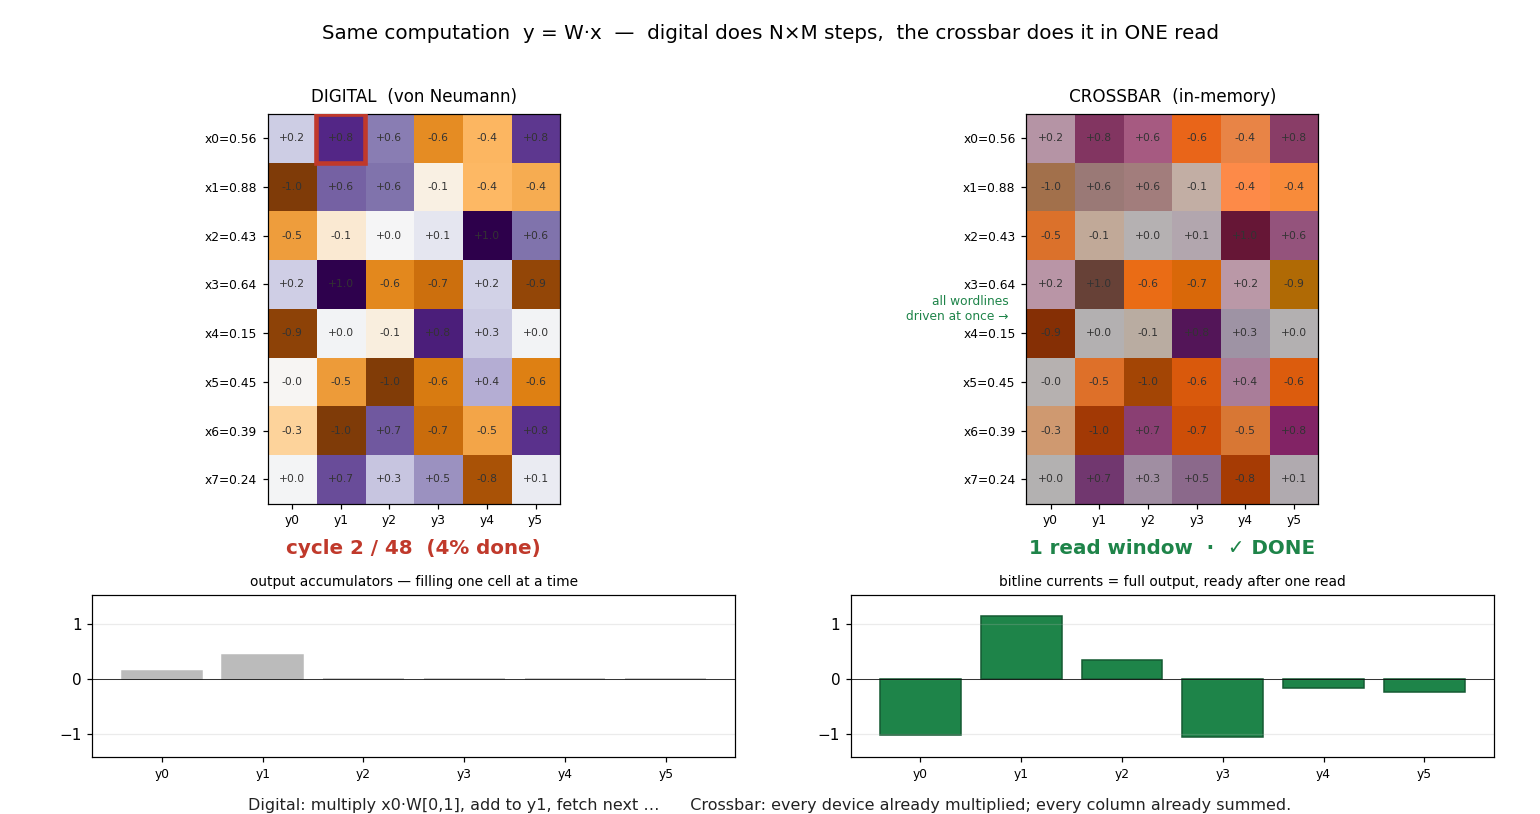
\includegraphics[width=0.32\textwidth]{figures/crossbar_parallel_f1.png}\hfill
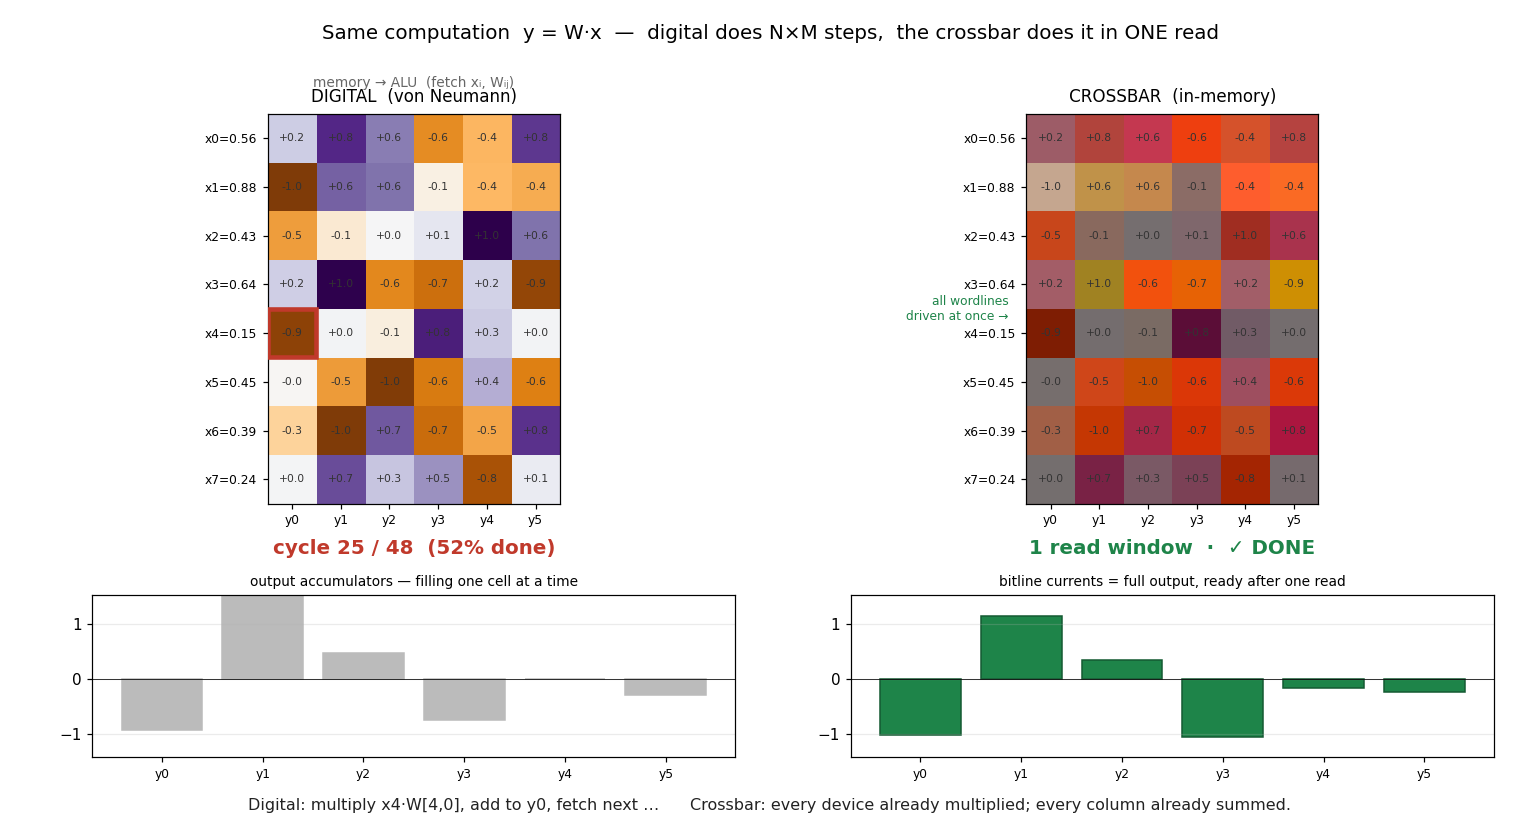
\includegraphics[width=0.32\textwidth]{figures/crossbar_parallel_f2.png}\hfill
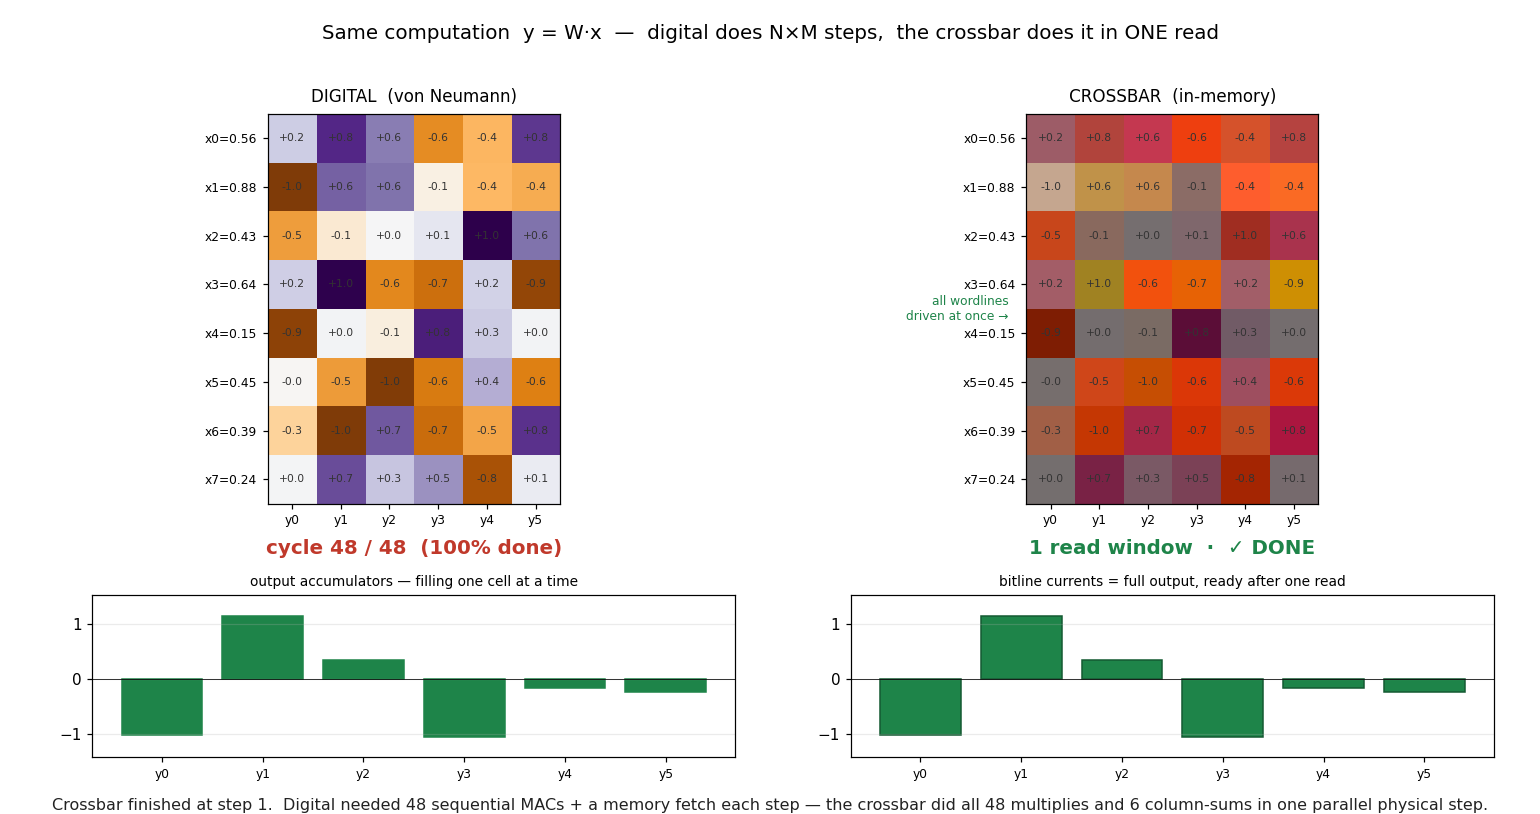
\includegraphics[width=0.32\textwidth]{figures/crossbar_parallel_f3.png}
\caption{The same MVM done two ways, shown at three times (left to right). The
digital engine steps through $N\times M$ multiply-accumulates with a memory fetch
each cycle (its counter climbs 1, mid, $N\times M$); the crossbar finishes the
whole product in one parallel read at step 1 and then holds the answer.}
\label{fig:parallel}
\end{figure*}

\begin{figure*}[t]
\centering
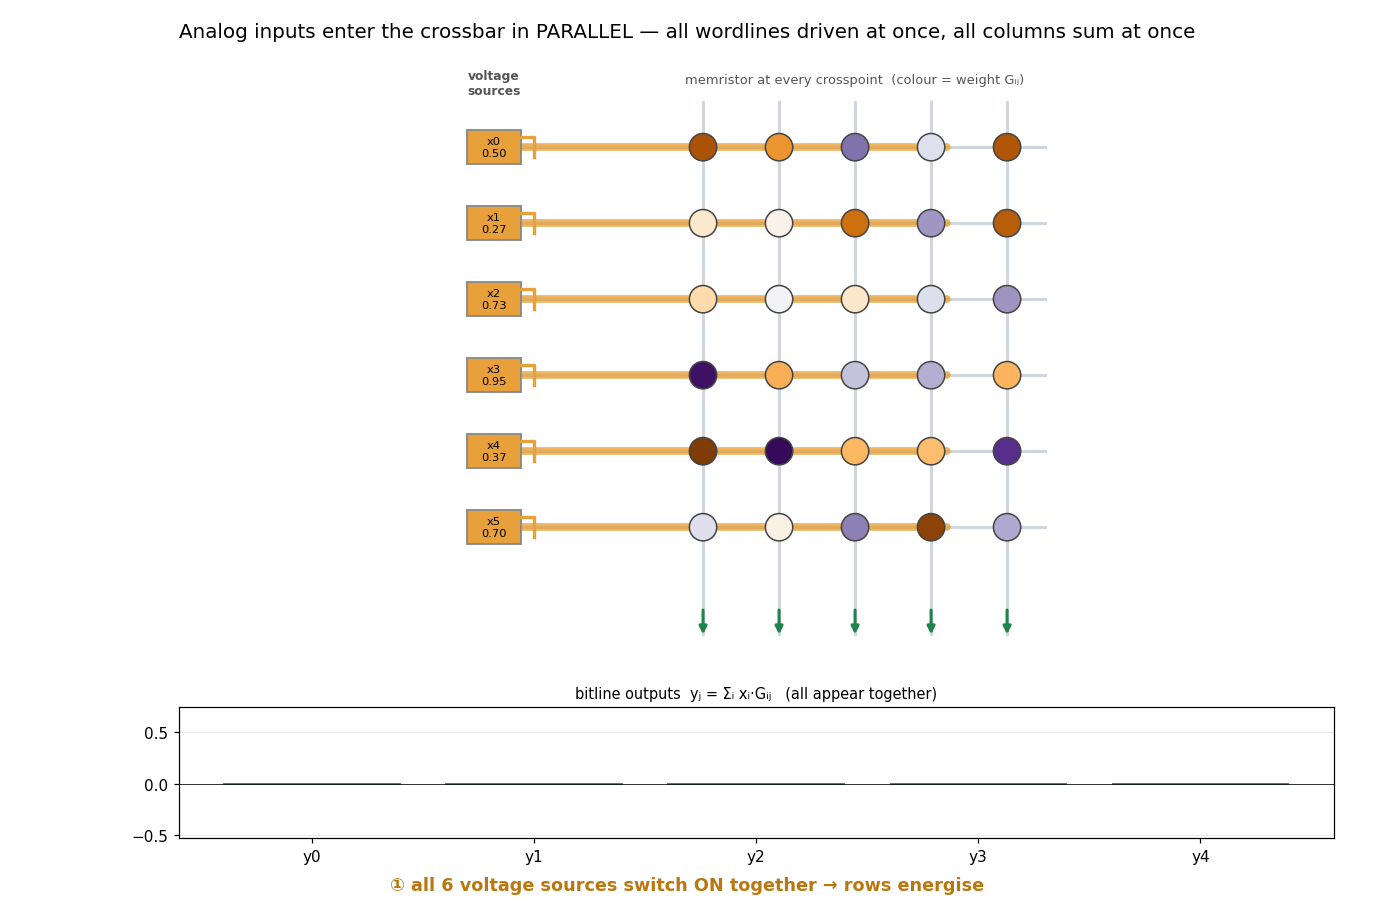
\includegraphics[width=0.32\textwidth]{figures/crossbar_circuit_f1.png}\hfill
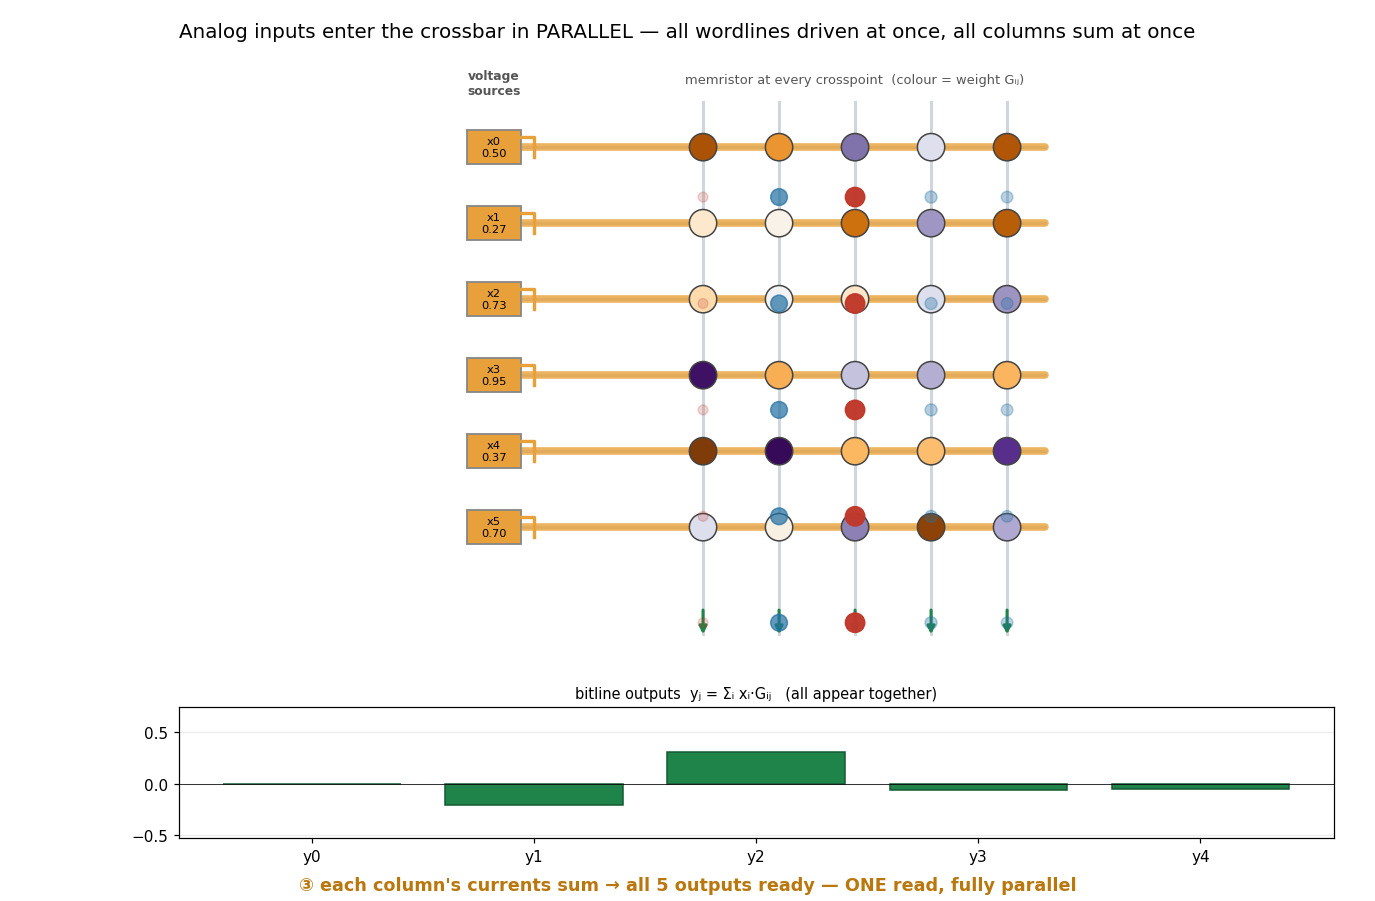
\includegraphics[width=0.32\textwidth]{figures/crossbar_circuit_f2.png}\hfill
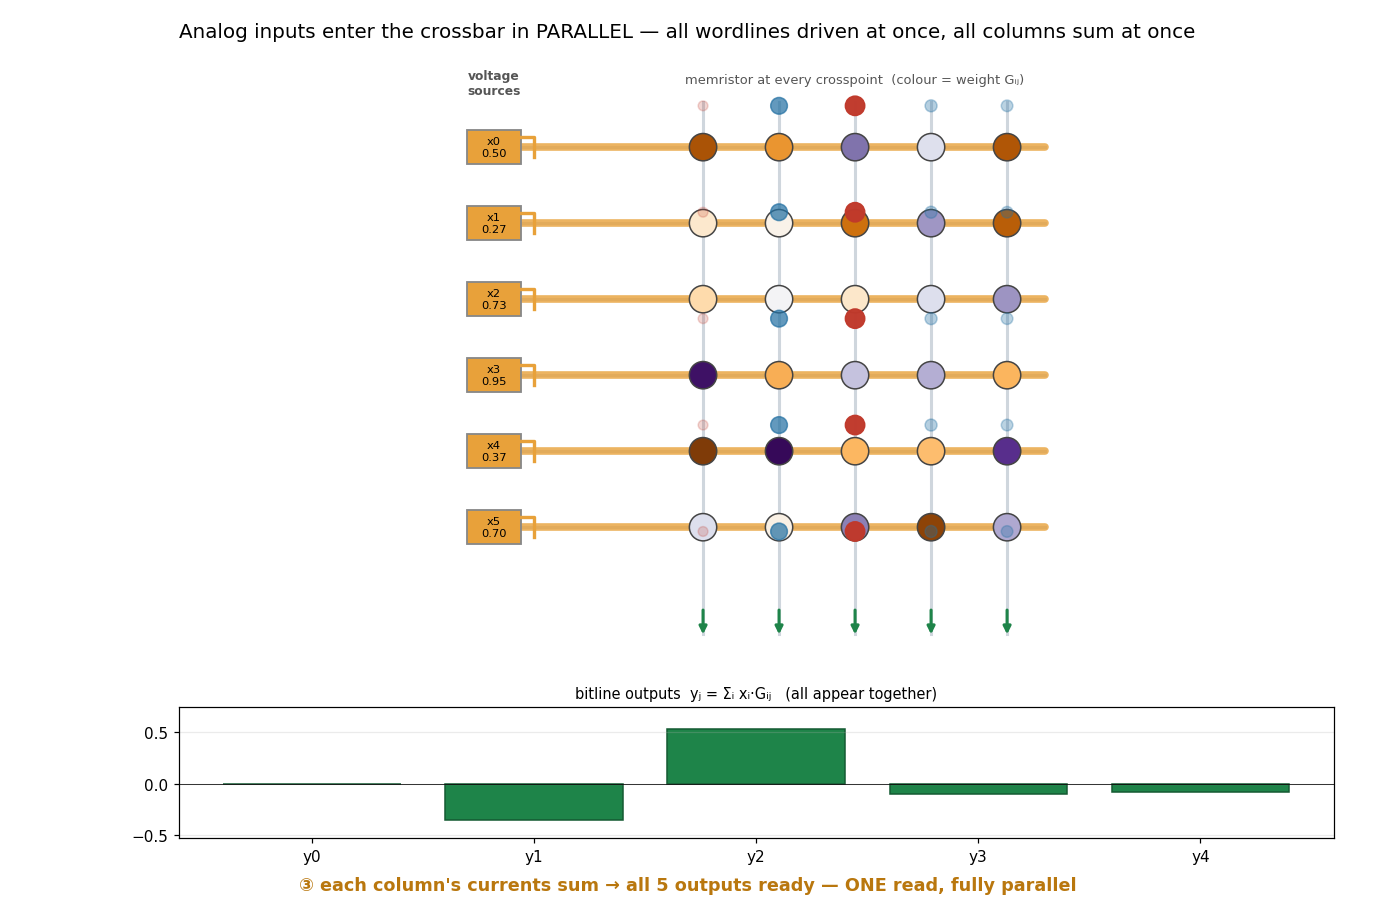
\includegraphics[width=0.32\textwidth]{figures/crossbar_circuit_f3.png}
\caption{Analog inputs entering the crossbar in parallel, shown at three times
(left to right): all wordlines are driven at once, every device passes $I=VG$,
and current then sums down every bitline simultaneously into the outputs.}
\label{fig:circuit}
\end{figure*}

\section{Reproducibility}
\label{app:repro}
All code accompanying this paper is in the public GitHub repository
\url{https://github.com/rayjyotir5/alox-crossbar-nonidealities} (Python 3.11;
NumPy, SciPy, scikit-learn, PyTorch, Matplotlib). It consists of three core
modules and several scripts:
\begin{itemize}
\item \texttt{alox\_crossbar.py}: device model, single-device sweep, 64x64 array
variability, image program/read, analog MVM (Fig.~\ref{fig:device}--\ref{fig:compute}).
\item \texttt{crossbar\_advanced.py}: vectorized MNA IR-drop solver, Arrhenius
retention, convolutional-layer fidelity, and the digit-classifier accuracy study
(Fig.~\ref{fig:inference}--\ref{fig:retention}, Tab.~\ref{tab:irdrop}).
\item \texttt{crossbar\_learn.py}: in-situ two-spiral training, hardware-in-the-loop
IR-drop training, and post-training retention (Fig.~\ref{fig:insitu}--\ref{fig:drift}).
\item \texttt{seeds\_experiments.py} and \texttt{harden2.py}: the multi-seed
study (classifier, in-situ on spirals and circles), the mixed-state IR-drop
table, the Arrhenius $E_a$ sensitivity, and the output-calibration baseline for
the IR-drop recovery. All headline numbers in the paper are produced here as
mean $\pm$ std over seeds.
\item Visualization scripts (\texttt{crossbar\_*\_viz.py}) produce the animations
whose stills appear in App.~\ref{app:extra}.
\end{itemize}
Each module is self-contained and writes its figures on execution; the full
pipeline runs in minutes on a single laptop CPU. Each headline result is reported
over multiple seeds (typically five for fast experiments, three for the slower
IR-aware training runs); the figures show a single representative seed while the
tables and text report the seed statistics.
